\section{Umsetzung}
In diesem Kapitel wird die Vorgehensweise der zuvor beschriebenen Problemstellungen erörtert.

\subsection{Aufbau der Testumgebung}



\subsubsection{Aufsetzen eines Nagios-Test-Systems}
Da die einzelnen Überwachungselemente in der Überwachungssoftware Nagios nach und nach eingetragen (/ definiert / assoziiert / verbunden) werden müssen, ist ein häufiges Neustarten der Nagios-Anwendung notwendig, damit die neuen Konfigurationsdateien übernommen werden.

Damit dies nicht auf dem bereits verwendetem Nagios-Server durchgeführt werden muss, wird ein Nagios-Testserver für diesen Zweck eingesetzt.

Da Nagios ein Unix-ähnliches Betriebssystem erfordert, wird für diesen Zweck die Linux-Distribution Debian als Betriebssystem des Testservers verwendet.

\subsubsection{Bilddatenbank als virtuelle Maschine}
Für die Simulation der verschiedenen Fehlerzuständen der einzelnen Überwachungselemente wird eine virtuelle Maschine mit einer \gls{OracleUCM} Prototypinstallation, die extra als Entwicklungsplattform erstellt wurde, verwendet.

\subsection{Übersicht Nagios-Agenten}
In diesem Unterkapitel werden die populärsten Agenten für Unix und Windows Betriebssysteme aufgelistet und nach den Punkten Sicherheit, subjektiver Aufwand für die Konfiguration und Art der Abfragemethode (aktiv oder passiv) verglichen.

\subsubsection{Unix-Agenten}
Für die auf Unix basierenden Betriebssysteme werden fünf verschiedene Möglichkeiten angeboten, die in Abbildung \ref{nagios-kern} als verschiedene Überwachungsmöglichkeiten von Nagios aufgelistet wurden.

%Tabelle Unix-Agenten


\begin{table}[h!]
\centering
\begin{threeparttable}[ht]
\begin{tabular}{l p{1.5cm} l p{1.5cm} l p{1.5cm} l p{1.5cm} l p{1.5cm} l p{1.5cm} p{1.5cm} p{1.5cm} p{1.5cm} p{1.5cm}}
 & \begin{turn}{50}\textbf{SSH}\end{turn} & \begin{turn}{50}\textbf{NRPE}\end{turn} & \begin{turn}{50}\textbf{SNMP}\end{turn} & \begin{turn}{50}\textbf{SNMP Traps}\end{turn} & \begin{turn}{50}\textbf{NSCA}\end{turn}\\ 
\hline
\textbf{Methode} & & & & & \\
\textit{aktiv} & \checkmark & \checkmark & \checkmark & - & - \\
\textit{passiv} & - & - & - & \checkmark & \checkmark\\
\textbf{Sicherheit} &  &  &  &  &  \\
\textit{Passwort} & - & - & \checkmark (v3) & \checkmark (v3) & -\\
\textit{Accesslist}\tnote{*} & \checkmark &  \checkmark & \checkmark (v2) & \checkmark (v2) & \checkmark \\
\textit{Verschlüsselung} &  \checkmark & \checkmark & \checkmark (v3) & \checkmark (v3) &  \checkmark \\
\textbf{Aufwand}\tnote{**} & \begin{footnotesize}leicht\end{footnotesize} & \begin{footnotesize}normal\end{footnotesize} & \begin{footnotesize}hoch\end{footnotesize} & \begin{footnotesize}hoch\end{footnotesize} & \begin{footnotesize}normal\end{footnotesize} \\
\end{tabular}
%\footnotesize
%* Einschränkung der Abfrage der Überwachungsinformationen anhand der \gls{IP}-Adresse
%\\
%** Subjektive Einschätzung
\begin{tablenotes}\footnotesize
      \item[*] Einschränkung der Abfrage der Überwachungsinformationen anhand der \gls{IP}-Adresse
        \item[**] Subjektive Einschätzung
    \end{tablenotes}
\caption{Übersicht der verschiedenen Unix-Agenten}
\end{threeparttable}
\end{table}




Dabei werden drei Agenten genannt, die eine aktive Ausführung der Nagios-Plugins benutzten.
Alle drei Agenten unterscheiden sich jedoch in den Punkten Sicherheit und Aufwand.
Der auf \gls{SSH} basierende Agent besitzt einen relativ geringen Aufwand für die Installation, da für den Aufbau der Kommunikation zwischen Nagios-Server und Client nur der öffentliche Schlüssel des Servers auf dem Client eingetragen werden muss.
Dadurch kann der Nagios-Server sich ohne Passwortabfrage an dem zu überwachendem Host anmelden und die sich darauf befindlichen Nagios-Plugins ausführen.
Da auf den meisten Unix-Servern bereits ein \gls{SSH}-Server läuft und deshalb kein weiterer Port geöffnet oder eine weitere Software installiert werden muss, ist diese Methode den anderen meist vorzuziehen.

Bei der \gls{NRPE}-Methode wird eine weitere Softwarekomponente auf dem Client installiert, die einen separaten Port für die Kommunikation mit dem Nagios-Server öffnet.
Wie bei dem Aufruf per \gls{SSH} müssen sich hier die Nagios-Plugins bereits auf dem Rechner befinden.
Dabei gilt als Unterschied dieser zwei ähnlichen Methoden zu beachten, dass für die Ausführung der Checks per \gls{SSH} ein extra Benutzerkonto auf dem Client erstellt werden muss und somit beliebige Systembefehle ausgeführt werden können, während die Ausführung von Kommandos bei \gls{NRPE} nur auf vorkonfigurierte Befehle beschränkt ist, wie in Kapitel \ref{sshnrpe} aufgeführt.
\label{unixagents}
Da \gls{SNMP} plattformunabhängig funktioniert ist es möglich diese Variante bei Unix- sowie bei Windowsservern einzusetzen.
Die verwendete \gls{SNMP}-Version bestimmt welche Sicherheitsmerkmale zur Verfügung stehen.
Zwar gibt es bereits seit Version 1 die Möglichkeit den Zugriff per Passwort in drei Gruppen aufzuteilen: kein Zugriff, Leserecht und Lese- mit Schreibrecht\footnote{Quelle: \cite{Barth08} S. 237}, jedoch wird dieses Passwort im Klartext übertragen, so dass es leicht auslesbar ist.
Auch die \gls{SNMP}-Version 2 inklusive der erweiterten Version 2c verwendet die gleiche unsichere Authentifizierung.
Erst ab Version 3 wird das Passwort verschlüsselt übertragen.
Während Barth behauptet, dass man bei \gls{SNMP} generell kein Passwort verwenden soll\footnote{Quelle: \cite{Barth08} S. 238}, da es leicht per Netzwerkmitschnittprogramme, wie WireShark, ausgelesen werden kann, wird in \cite{Jose07} S. 121 klargestellt, dass die Version 3 eine verschlüsselte Authentifizierung durch den MD5- oder SHA-Algorithmus ermöglicht.

Die passive Variante über \gls{SNMP} bei der der Client die Ergebnisse der Checks an den Nagios-Server sendet, auch \gls{SNMP}-Traps genannt, funktioniert nach dem gleichen Prinzip.
Da das Auslesen der \gls{MIB} per \gls{SNMP} im Gegensatz zu den anderen Varianten deutlich komplexer ist, wird der Aufwand als hoch eingestuft.

Ein weiterer Vertreter, der passive Checks ermöglicht, ist der \gls{NSCA}-Agent.
Wie die anderen Unix-Agenten bietet es die Möglichkeit den Datenaustausch zwischen Nagios-Server und Client zu verschlüsseln.
Alle Unix-Agenten erlauben es den Zugriff auf die Nagios-Plugins auf bestimmte \gls{IP}-Adressen zu beschränken.
Die Liste mit diesen \gls{IP}-Adressen nennt man auch \textit{Accesslist}.

\subsubsection{Windows-Agenten}
Da die zu überwachende Oracle UCM Anwendung auf einem Windows-Server betrieben wird und die bereits vorgestellten Agenten mit Ausnahme der \gls{SNMP}-Varianten nur unter Unix einsetzbar sind, müssen zusätzlich die explizit für Windows entwickelten Nagios-Agenten untersucht werden.
Dabei wird die Auswahl der Kandidaten auf vier Bewerber beschränkt, siehe Tabelle \ref{tab:winagents}.
%Tabelle Windows-Agenten
%\vspace{1.6cm}
\begin{table}[!cht]
\centering
\begin{threeparttable}
\begin{tabular}{l p{1.3cm} l p{1.3cm} l p{1.3cm} l p{1.3cm} l p{1.3cm} l p{1.3cm} p{1.3cm} p{1.3cm} p{1.3cm} p{1.3cm}}
 & \begin{turn}{50}\textbf{NSClient}\end{turn} & \begin{turn}{50}\textbf{NRPE\_NT}\end{turn} & \begin{turn}{50}\textbf{NC\_net}\end{turn} & \begin{turn}{50}\textbf{NSClient++}\end{turn} & \begin{turn}{50}\textbf{OpMon Agent}\end{turn}\\ 
\hline
\textbf{Methode} & & & & & \\
\textit{aktiv} & \checkmark & \checkmark & \checkmark & \checkmark & \checkmark\\
\textit{passiv} & - & - & \checkmark & \checkmark & -\\
\textit{NSClient}\tnote{1} & \checkmark & - & \checkmark & \checkmark & \checkmark\\
\textit{NRPE}\tnote{2} & - & \checkmark & \checkmark & \checkmark & \checkmark\\
\textbf{Sicherheit} &  &  &  &  &  & \\
\textit{Passwort} & \checkmark & \checkmark & - & \checkmark & \checkmark\\
\textit{Accesslist}\tnote{3} & - & - & \checkmark & \checkmark & \checkmark\\
\textit{Verschlüsselung} & - & \checkmark & \checkmark & \checkmark & -\\
\textbf{Aufwand}\tnote{4} & \begin{footnotesize}normal\end{footnotesize} & \begin{footnotesize}hoch\end{footnotesize} & \begin{footnotesize}normal\end{footnotesize} & \begin{footnotesize}normal\end{footnotesize} & \begin{footnotesize}normal\end{footnotesize}\\
\end{tabular}
\begin{tablenotes}\footnotesize
		\item[1] Kompatibilität mit dem NSClient-Dienst
		\item[2] Erlaubt Ausführung von vorkonfigurierten Kommandos
        \item[3] Einschränkung der Abfrage der Überwachungsinformationen anhand der \gls{IP}-Adresse
        \item[4] Subjektive Einschätzung
    \end{tablenotes}
\caption{Übersicht der verschiedenen Windows-Agenten}
\label{tab:winagents}
\end{threeparttable}
\end{table}
\newpage
Der NSClient-Dienst liefert die Möglichkeit lokale Windows-Ressourcen über das Netzwerk mit eigenem Port (Standport 1248) abzufragen.
Das Plugin \textit{check\_nt} wurde explizit für diesen NSClient-Dienst entwickelt und steht durch die Nagios-Plugins standardmäßig zur Verfügung.
Dadurch können die grundlegende Informationen für die Systemüberwachung aus Kapitel \ref{syschecks}, wie Zustände von Prozesse, Services, CPU-Auslastung, Festplattenplatz, usw. abgefragt werden.
Der Zugriff auf den NSClient-Dienst per \textit{check\_nt} wird in Abbildung \ref{fig:cknt} gezeigt.
\begin{figure}[ht]
	\centering
	   \fbox{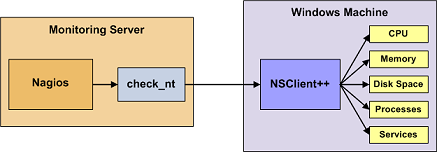
\includegraphics[width=0.8\textwidth]{bilder/monitoring-windows.png}}
		\caption[Abfrage von Windows-Ressourcen durch \textit{check\_nt}]{Abfrage von Windows-Ressourcen durch \textit{check\_nt}\protect\footnote}
		\label{fig:cknt}
\end{figure}
\footnotetext{Quelle: \url{http://nagios.sourceforge.net/docs/3\_0/images/monitoring-windows.png}}

Diese Abfrage kann durch die Ausführung auf der Kommandozeile getestet werden:

\begin{figure}[ht]
	\centering
	   \fbox{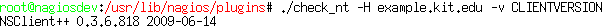
\includegraphics[width=0.75\textwidth]{bilder/check_nt-stdp.png}}
		\caption{Zugriff auf den NSClient-Dienst durch check\_nt}
		\label{fig:ckntsh}
\end{figure}

Der erste und zugleich älteste Agent NSClient wird nicht mehr aktiv entwickelt und ist als aktuellste Version 2.0.1 aus dem Jahre 2003 bereits recht alt.
Daher wird auch keine Verschlüsselung der ein- und ausgehenden Daten unterstützt.
Auch bietet NSClient keine Möglichkeit aktiv vom Nagios-Server aus Nagios-Plugins oder weite Programme auszuführen, die sich auf dem zu überwachendem Host befinden.

Um dies auch für Windows-Server zu ermöglichen gibt es eine auf Windows portierte \gls{NRPE}-Variante, die sich NRPE\_NT nennt.
Hier lassen sich die Plugins direkt über den Nagios-Server aufrufen und die ausgetauschten Informationen werden verschlüsselt über das Netzwerk übertragen.

Beide bisher genannte Windows-Agenten bieten keine Möglichkeit eine \textit{Accesslist} anzulegen, erst das Programm NC\_net bietet diese Möglichkeit inklusive dem Sicherheitsmerkmal Verschlüsselung an.
Außerdem können durch den eingebauten \gls{NRPE}-Dienst aktiv Nagios-Plugins auf dem Client aufgerufen werden.
Als Besonderheit lassen sich durch NC\_net sowohl aktiv als auch passiv Testergebnisse an den Nagios-Server übertragen. 

Der Nagios-Agent NSClient++ besitzt diesselben Merkmale wie NC\_net, jedoch kann der Nagios-Server noch über ein Passwort zusätzlich verifiziert werden.

Die Möglichkeit Informationen per \gls{SNMP} und \gls{SNMP}-Traps abzufragen ist auch unter Windows möglich.
Dabei gelten die gleichen Richtlinien, Hinweise und Einschränkungen wie zuvor in Kapitel \ref{unixagents} aufgeführt.

\subsubsection{Auswahl und Konfiguration des Nagios-Agenten}

\paragraph{Auswahl}
Anhand der im vorherigen Kapitel beschriebenen Übersicht der Windows-Agenten und der daraus resultierenden Übersichtstabelle \ref{tab:winagents} wird ein geeigneter Kandidat für die Testumgebung ausgewählt.
Da nur ein Windows-Agent alle drei Sicherheitsmerkmale anbietet und dabei aktive und passive Überwachungsmethoden erlaubt, fällt die Wahl auf das Programm \textbf{NSClient++}.

\paragraph{Installation und Konfiguration}

Der Nagios-Agent NSClient++ kann im Gegensatz zu den meisten anderen Windows-Agenten komfortabel über einen graphischen Benutzerdialog installiert werden.
Während des Installationsvorgangs kann auch festgelegt werden welche Komponenten installiert werden sollen.
Dabei werden diese Komponenten nicht standardmäßig geladen, sondern im nächsten Dialogfenster auswählbar:

\begin{figure}[ht]
	\centering
	   \fbox{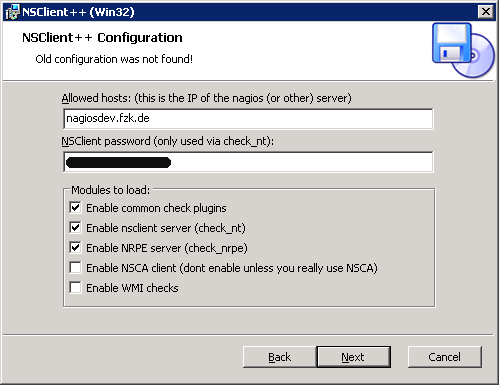
\includegraphics[width=0.55\textwidth]{bilder/nsc2.png}}
		\caption{Konfiguration des NSClient++ während der Installation}
		\label{nscs2}
\end{figure}

Außerdem können direkt während der Installation die \gls{IP}-Adresse bzw. der \gls{FQDN} des Nagios-Servers und das gewünschte Passwort eingetragen werden.

Durch die während des Installationsprozesses geladenen Komponenten für den NSClient- und \gls{NRPE}-Dienst können die Standard-Nagios-Plugins \textit{check\_nt} und \textit{check\_nrpe} mit dem Windows-Server verwendet werden.
Dabei läuft die Kommunikation zwischen dem Nagios- und dem Windows-Server folgendermaßen ab:

\begin{figure}[ht]
	\centering
	   \fbox{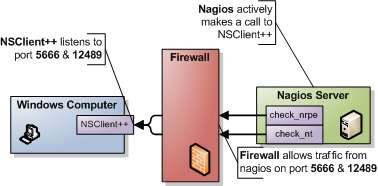
\includegraphics[width=0.7\textwidth]{bilder/nagios-active-nsclient-and-nrpe.png}}
		\caption[Kommunikation zwischen Nagios und NSClient++]{Kommunikation zwischen Nagios und NSClient++\protect\footnote}
		\label{nscs2}
\end{figure}
\footnotetext{Quelle: \cite{NSClient}}
%http://nsclient.org/nscp/raw-attachment/wiki/doc/usage/nagios/nagios-active-nsclient.png

Bei Windows-Server mit vielen Verbindungen und Diensten können Remote Procedure Calls (\gls{RPC}), bei denen dynamisch Ports ab 1025 verwendet werden, bereits den Standardport des NSClient-Dienstes (1248) unter Umständen bereits vor dem Start des Dienstes belegen.\footnote{Quelle: \cite{Barth08} S. 481}
Um dies zu verhindern wurde der Port des NSClient-Dienstes beim NSClient++ bereits vom Entwickler auf einen höheren Port (12489) gewechselt.

Alle bisherigen Einstellungen können in der Konfigurationsdatei \textit{NSC.ini}, die sich in dem Installationsverzeichnis des NSClient++ befindet, verändert werden.
In dieser Datei befinden sich noch mehr Einstellungsmöglichkeiten; im Folgenden werden nur für die Umsetzung relevanten (notwendig essentiell benötigten) Parameter aufgelistet.

\begin{lstlisting}[captionpos=b, caption=NSClient++ Konfigurationsdatei, label=code:nsc, breaklines = true, language=sh]
;# NSCLIENT PORTNUMMER
;#  Die Portnummer des NSClient-Dienstes
port=13596

;# NRPE PORTNUMMER
;#  Die Portnummer des NRPE-Dienstes
port=13597

;# SSL SOCKET
;#  Die Aktivierung von SSL der Kommunikation zwischen Nagios- und Windows-Server 
use_ssl=1

;# NRPE BEFEHLSDEFINITIONEN
;# Definitionen der Befehle, die durch den NRPE-Dienst aufrufbar sind
check_uname=scripts\check_uname.exe
check_reflog=scripts\check_logfiles.exe -f scripts\logfile.cfg
\end{lstlisting}

Damit die vorgenommen Änderung übernommen werden, muss der Dienst des NSClient++ neu gestartet werden. 

%\begin{figure}[ht]
%	\centering
%	   \fbox{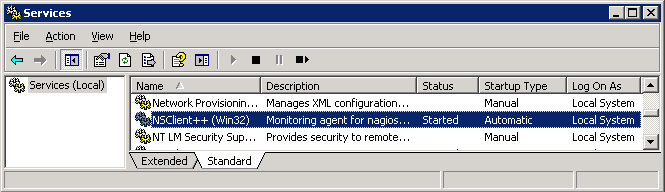
\includegraphics[width=0.85\textwidth]{bilder/nsc3.png}}
%		\caption{NSClient++ Windowsdiensteintrag}
%		\label{nscs3}
%\end{figure}

Durch das Ausweichen auf höher gelegene Portnummern können die zuvor genannten Probleme aufgrund der \gls{RPC}s verhindert werden.

Der bereits höher liegende Standardport des NSClient-Dienstes beim NSClient++ wird zusätzlich noch abgeändert, damit die Tatsache, dass sich ein Nagios-Agent auf dem Computer befindet, nicht sofort ersichtlich ist.
Dieser sicherheitstechnische Aspekt wurde bereits in Kapitel \ref{changeport} behandelt.

Damit die \gls{SSL}-Verschlüsselung zwischen den Servern aktiviert wird, muss man es explizit in der Konfigurationsdatei mit der Option \textit{use\_ssl=1} angeben.

Die Definitionen der \gls{NRPE}-Kommandos dienen dafür, dass durch den Nagios-Server per \textit{check\_nrpe} mit dem Befehlsnamen der darauf folgende Befehl ausgeführt wird.

Aufgrund der abgeänderten Portnummer muss man den Port bei dem Aufruf explizit angeben.
Ein Aufruf eines solchen \gls{NRPE}-Kommandos vom Nagios-Server wird in der folgenden Abbildung gezeigt:

\begin{figure}[ht]
	\centering
	   \fbox{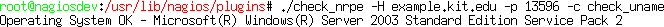
\includegraphics[width=0.85\textwidth]{bilder/nrpe-check.png}}
		\caption{Aufruf eines NRPE-Kommandos}
		\label{nrpecheck}
\end{figure}



Anhand des Befehlsnamens \textit{check\_uname} führt der \gls{NRPE}-Dienst die in der Konfigurationsdatei eingetragene Datei \textit{check\_uname.exe} aus.

Der Aufruf um Informationen durch den NSClient-Dienst abzufragen sieht ähnlich aus:

\begin{figure}[ht]
	\centering
	   \fbox{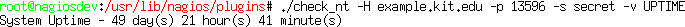
\includegraphics[width=0.85\textwidth]{bilder/nsclient-check.png}}
		\caption{Aufruf des NSClient-Dienstes}
		\label{ntcheck}
\end{figure}

Die Servicedefinition des vorherigen NSClient-Aufrufs muss wie nachfolgend/folgt in der Nagios-Konfiguration eingetragen:
\begin{lstlisting}[captionpos=b, caption=Servicedefinition des NSClient-Checks, label=nt-servdef, breaklines = true, language=sh]
define service{
        use                     generic-service
        host_name               example.kit.edu
        service_description     Uptime
        check_command           check_nt!-p 13596 -s secret -v UPTIME
        }
\end{lstlisting}

Damit nicht jeder einzelne Serviceeintrag abgeändert werden muss, falls sich der Port oder das Passwort des zu überwachenden Computers ändert, können eigene Befehlsdefinitionen erstellt werden.

\begin{lstlisting}[captionpos=b, caption=Server spezifische Befehlsdefinition, label=cus-nt-servdef, breaklines = true, language=sh]        
define command{
        command_name    check_nt_example
        command_line    /usr/lib/nagios/plugins/check_nt -H $HOSTNAME$ -p 13597 -p secret -v $ARG1$
        }
\end{lstlisting}

Dadurch muss nur diese Befehlsdefinition bei einer Änderung bearbeitet werden.
Die vorherige Servicedefinition in Listing \ref{ntcheck} kann dann in verkürzter Form eingetragen werden:

\begin{lstlisting}[captionpos=b, caption=Verkürzte Servicedefinition des NSClient-Checks, label=nt-servdef, breaklines = true, language=sh]
define service{
        use                     generic-service
        host_name               example.kit.edu
        service_description     Uptime
        check_command           check_nt_example!UPTIME
        }
\end{lstlisting}




\subsection{Umsetzung der Systemüberwachung}

Die in Kapitel \ref{syschecks} aufgelisten Prozesse und Services können durch den NSClient-Dienst vom Nagios-Server überwacht werden.
Dafür wird der in Listing \ref{cus-nt-servdef} definierte verkürzte Befehl für \textit{check\_nt} benutzt.

\begin{lstlisting}[captionpos=b, caption=Prozess- und Service-Check Servicedefintionen, label=procservdef, breaklines = true, language=sh]
#Prozess des IIS Webservers
define service{
        use                     generic-service
        host_name               example.kit.edu
        service_description     IIS Prozess
        check_command           check_nt_example!PROCSTATE -l w3wp.exe
        }

#Zeitdienst
define service{
        use                     generic-service
        host_name               example.kit.edu
        service_description     Zeitdienst
        check_command           check_nt_example!SERVICESTATE -l W32TIME
        }
\end{lstlisting}

Mit diesen zwei Einträgen wird der Prozess des \gls{IIS}-Webservers und der Status des Dienstes zum Zeitabgleich überwacht.
Andere Prozesse und Dienste lassen sich nach dem gleichen Schema überwachen.

Nach einem Neustart von Nagios werden beide Einträge im Webinterface angezeigt:

\begin{figure}[ht]
	\centering
	   \fbox{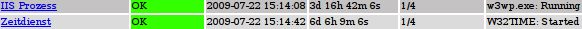
\includegraphics[width=0.95\textwidth]{bilder/servproc.png}}
		\caption{Prozess- und Dienstüberwachung im Nagios-Webinterface}
		\label{servprocgui}
\end{figure}

Die Festplattenspeicherausnutzung und die Prozessorauslastung wird auf ähnliche Weise überwacht.
Hierbei muss beachtet werden, dass die Testergebnisse nicht eindeutig sind, im Gegensatz zu der Service- und Prozessüberwachung.
Wann Nagios alarmieren soll muss vom Anwender in Form von Parametern festgelegt werden.

\begin{lstlisting}[captionpos=b, caption=Überwachung der Festplatten- und Prozessorauslastung, label=cpuhdddef, breaklines = true, language=sh]
#Belegung der Partition C:
define service{
        use                     generic-service
        host_name               example.kit.edu
        service_description     C:\ Drive Space
        check_command           check_nt_example!USEDDISKSPACE -l c -w 85 -c 100
        }
        
#CPU Auslastung der letzten 5 Minuten
define service{
        use                     generic-service
        host_name               example.kit.edu
        service_description     CPU Load
        check_command           check_nt_example!CPULOAD -l 5,80,100
        }
\end{lstlisting}

Für diese Festplattenüberwachung versendet Nagios eine Warnung, wenn der belegte Speicherplatz auf der C-Partition die 85\% Marke überschreitet und meldet einen kritischen Fehler bei 100\%.
Bei der Prozessorüberwachung schlägt Nagios Alarm, wenn der Mittelwert der Auslastung in den letzten fünf Minuten mehr als 80\% bzw. 100\%  betragen hat.


\subsection{Umsetzung der Funktionlitätstest}

Für die Ausführung der einfachen Funktionlitätstest aus Kapitel \ref{funztest} werden Benutzerinformationen zur Anmeldung benötigt.
Nagios besitzt extra hierfür die Möglichkeit diese Benutzerinformationen in Variablen zu speichern, damit sie nicht einzeln bei jeder Servicedefinition verändert werden müssen.
Da sich die Definition dieser Variablen in einer externen Datei befindet, können die Zugriffsrechte auf diese Datei eingeschränkt werden, wodurch die Anmeldedaten bei den Servicedefinitionen nicht auslesbar sind.

\begin{lstlisting}[captionpos=b, caption=Funktionalitätstest der Benutzeranmeldung, label=userauthdef, breaklines = true, language=sh]
#Anmeldung an Oracle UCM mit lokalem Benutzerkonto
define service{
        use                     generic-service
        host_name               example.kit.edu
        service_description     Anmeldung Oracle UCM als lokaler Benutzer
        check_command           check_http!-u "/bdb/idcplg?IdcService=LOGIN&Action=GetTemplatePage&Page=HOME\_PAGE&Auth=Internet"  -a $USER3$:$USER4$ -e "Sie sind angemeldet als" -S
        }
\end{lstlisting}


Dabei werden dem Nagios-Plugin \textit{check\_http} mit dem \pictext{u}-Parameter die URL zur Benutzeranmeldungseite und mit dem Parameter \pictext{a} der Benutzername und -passwort mitgegeben.
Der nach dem Parameter \pictext{e} folgende String wird dann in der Antwort des Servers gesucht.
Sollte dieser String nicht gefunden werden ist die Authentifizierung fehlgeschlagen und es wird durch Nagios eine Meldung versendet.
Mit dem Parameter \pictext{S} wird angegeben, dass eine \gls{SSL}-verschlüsselte Verbindung zum Webserver über HTTPS hergestellt werden soll, ansonsten würden die Benutzerinformationen im Klartext übertragen werden, wodurch sie leicht für Angreifer auslesbar wären.

Für das Auslesen von Informationen aus der Statusseite der Oracle UCM-Anwendung wurde ein einfaches BASH-Script entwickelt:

\begin{lstlisting}[captionpos=b, caption=Auslesen der Verbindungen zur Datenbank, label=dbcon, breaklines = true, language=sh]
#!/bin/bash
E_BADARGS=2
if [ ! -n "$6" ]
then
        echo "Usage: `basename $0` -url <URL> -u <username> -p <password>"
        exit $E_BADARGS
fi

DBCONNECTIONS=$(wget -qO-  --user $4 --password $6 $2 | grep "System Database")
DBCONNECTIONS=${DBCONNECTIONS##*>}
DBCONNECTIONS=${DBCONNECTIONS%% *}
echo $DBCONNECTIONS
\end{lstlisting}

Dabei muss als URL die Seite mit den Datenbankverbindungen und gültige Benutzerinformationen mitgegeben werden.
Anschließend wird die aufgerufene Seite nach der gewünschte Informationen untersucht und ausgegeben.

Dieses einfaches Script kann auch dazu verwendet um andere Informationen von der Statusseite abzufragen.

\subsection{Auswertung der Logdateien}

Um die drei genannten Logdateien aus Kapitel \ref{checklog} auszuwerten wird durch den \gls{NRPE}-Dienst das Plugin \textit{check\_logfiles} von Gerhard Laußer eingesetzt.

Dieses Plugin besitzt bereits einige nützliche Funktionen für die Überwachung von Logdateien.
Durch das Setzten eines Zeitstempels filtert das Plugin veraltete Einträge heraus und untersucht nur neu hinzugekommene Zeilen.
Der Rotationsalgorithmus der Oracle UCM-Logdateien kann dem Plugin durch die Verwendung einer Konfigurationsdatei mitgeteilt werden.

Die Konfigurationsdatei für das \textit{check\_logfiles}-Plugin wird im folgendem Listing gezeigt:


\begin{lstlisting}[captionpos=b, caption=Konfigurationsdatei für \textit{check\_logfiles}, label=chklogcfg, breaklines = true, language=sh]
@searches = ({
  tag => 'ucmlogs',
  type => 'rotating::uniform',
  logfile => 'D:/bdb2/weblayout/groups/secure/logs/bdb/IdcLnLog.htm',
  rotation => 'refinery\d{2}\.htm',
  warningpatterns => [
        'Cannot identify file',
	  'Bad CRC value in IHDR chunk',
	  'Der Dateiname darf nicht länger als 80 Zeichen sein',
    ],
});
\end{lstlisting}

Mit dem \pictext{tag}-Attribut wird diese Auswertung eindeutig identifizierbar gemacht, da man in der gleichen Konfigurationsdatei mehrere Logdateien bzw. weitere Durchsuchungen definieren kann.
Das Attribut \pictext{type} muss hier so gesetzt werden, da die aktuelle Logdatei und die wegrotierte Logdatei das gleichen Namensschema benutzten.
Der Pfad zu den Logdateien wird über das Attribut \pictext{logfile} gesetzt.
Da die einzelnen Logdateien mit einem bestimmten Namensmuster erstellt werden (siehe Kapitel \cite{checklog}), muss dieses Namensmuster hier direkt angegeben werden.
In diesem Falle durchsucht das \textit{check\_logfiles}-Plugin alle Logdateien mit dem Namen \textit{refinery00.htm} bis \textit{refinery99.htm}.
Alle gefundenen Dateien werden dem Datum nach sortiert und die aktuellste Datei wird untersucht.
Nach welchen Stopwörtern gesucht werden soll wird mit dem Attribut \pictext{warningpatterns} angegeben, sofern mindestens einer dieser Strings gefunden wurde liefert das Plugin ein WARNING als Rückmeldung inklusive der Zeile in dem das Stopwort gefunden wurde.

\begin{figure}[ht]
	\centering
	   \fbox{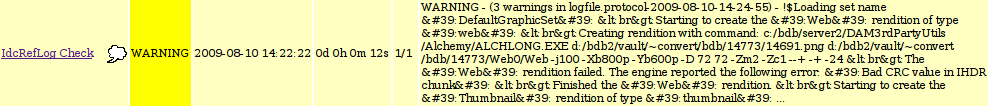
\includegraphics[width=0.95\textwidth]{bilder/logcheckwarn.png}}
		\caption{Ausgabe der betreffenden Zeile in der Logdatei}
		\label{checklogwarn}
\end{figure}


\subsection{Benutzersimulation}

Um die Funktionalität der Anwendung eindeutig festzustellen werden typische Benutzeraktionen simuliert und die Ergebnisse an Nagios übermittelt.

Solche typische Aktionen sind das Einchecken eines Bildes, Suche nach einem Bild und schließlich die Anforderung des Originalbildes und der konvertierten Bilder.
%Benutzertätigkeiten, Handlungen
Da Nagios standardmäßig ein Plugin periodisch jede fünf Minuten aufruft, würde sich die Festplatte und die Datenbank des \gls{OracleUCM}-Servers im Laufe der Zeit an ihre Kapazitäten stoßen.
Daher werden nach der Anforderung und Überprüfung der Bilder alle Testbilder vom Server entfernt.

Der Ablauf der Benutzersimulation soll in verkürzter Form durch folgendes Struktogramm verdeutlicht werden:

\begin{figure}[ht]
	\centering
	   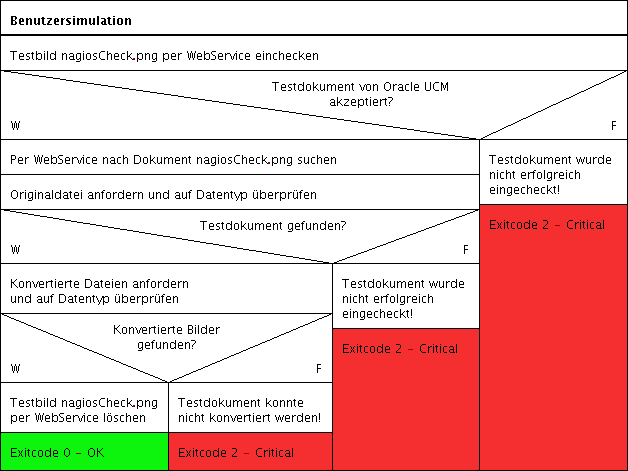
\includegraphics[width=0.9\textwidth]{bilder/Benutzersimulation.png}
		\caption{Geplanter Ablauf der Benutzersimulation}
		\label{user-sim}
\end{figure}



Per Webservice soll ein Testbild an den Server geschickt und eingecheckt werden.
In diesem ersten Schritt wird auch gleichzeitig die Erreichbarkeit der Anwendung über das Netzwerk getestet.

Wenn die Übertragung des Bildes erfolgreich wird anschließend nach dem soeben eingecheckten Bild per Dateinamen gesucht um die Funktionalität der Indizierung zu kontrollieren.

Sollte das Bild gefunden werden, wird es vom Nagios-Server angefordert und auf seine Korrektheit überprüft.
Der gleiche Test wird mit den konvertieren Bildversion durchgeführt, um die Funktion der Konvertierung zu überwachen.

Falls alle Tests erfolgreich waren, wird das Testbild und alle konvertierten Bilder vom \gls{OracleUCM}-Server gelöscht.
Bei den anderen Szenarien gibt das Plugin den Wert 2 für den Status CRITICAL zurück.\\

Die Realisierung dieser Simulation wird durch zwei Plugins realisiert.

Das erste Plugin dient zum Einchecken des Testbildes.
Dabei ruft der Nagios-Server ein auf PHP-basierendes Script auf.
In diesem Script wird die PHP-Klasse \textit{nuSOAP} eingebunden, damit man vereinfacht auf Web Services zugreifen kann.
Die Kommunikation zwischen Client und Server bei der Benutzung eines Web Services findet im \gls{XML}-Format statt.
Um den Aufwand zu vermeiden diese \gls{XML}-Datei immer selbst zu erstellen, wird mit Hilfe der \gls{WSDL}-Datei auf dem \gls{OracleUCM}-Server die benötigten Parameter beim Aufruf eines Web Services von \textit{nuSOAP} ausgelesen.

\begin{figure}[ht]
	\centering
	   \fbox{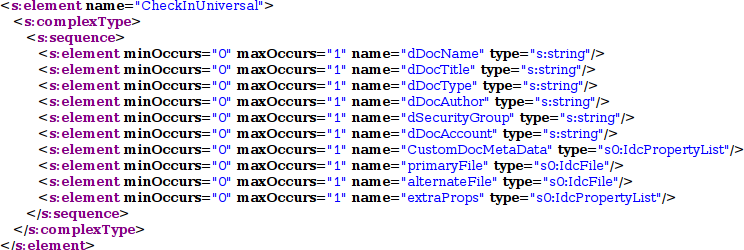
\includegraphics[width=0.9\textwidth]{bilder/wsdlscrn.png}}
		\caption{Anforderungsparameter aus der WSDL-Datei}
		\label{wsdl1}
\end{figure}


%\begin{lstlisting}[captionpos=b, caption=Anforderungsparameter aus der WSDL-Datei, label=1stwsdl, breaklines = true, language=xml]
%<s:element name="CheckInUniversal">
% <s:complexType>
%  <s:sequence>
%   <s:element minOccurs="0" maxOccurs="1" name="dDocTitle" type="s:string"/>
%   <s:element minOccurs="0" maxOccurs="1" name="dDocType" type="s:string"/>
%   <s:element minOccurs="0" maxOccurs="1" name="dDocAuthor" type="s:string"/>
%   <s:element minOccurs="0" maxOccurs="1" name="dSecurityGroup" type="s:string"/>
%   <s:element minOccurs="0" maxOccurs="1" name="dDocAccount" type="s:string"/>
%   <s:element minOccurs="0" maxOccurs="1" name="primaryFile" type="s0:IdcFile"/>
%  </s:sequence>
% </s:complexType>
%</s:element>
%\end{lstlisting}

\begin{lstlisting}[captionpos=b, caption=Anforderungsparameter des ersten Plugins, label=1stplugin, breaklines = true, language=php]
$ergebnis = $soap->CheckInUniversal(array(
 'dDocAuthor'=>$stellentuser,
 'dDocTitle'=>$page['title'],
 'dSecurityGroup'=>$page['stellent_secgroup'],
 'dDocAccount'=>$page['stellent_konto'],
 'dInDate'=>date("d.m.y H:i"),
 'dDocType'=>$page['stellent_docType'],
 'doFileCopy'=>'1',
 'dDocFormat'=>'image/png',
 'primaryFile'=>array(
	'fileName'=>$page['title'],
	'fileContent'=>$content)
));

\end{lstlisting}


Dafür enthält das erste PHP-Script die URL zu der \gls{WSDL}-Datei für den Web Service \textit{CheckInUniversal}.
Durch diese \gls{WSDL}-Datei

\begin{figure}[ht]
	\centering
	   \fbox{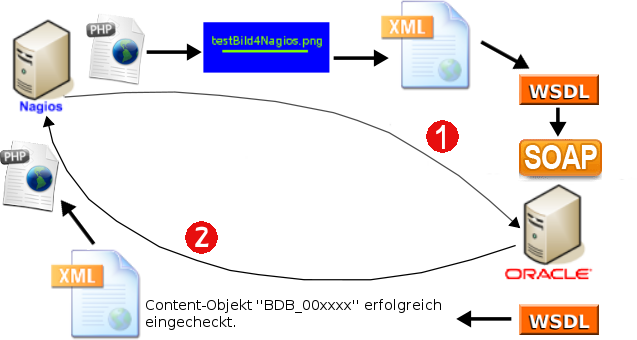
\includegraphics[width=0.93\textwidth]{bilder/wsdl.png}}
		\caption{Technischer Ablauf der Benutzersimulation}
		\label{usersim}
\end{figure}



\begin{figure}[ht]
	\centering
	   \fbox{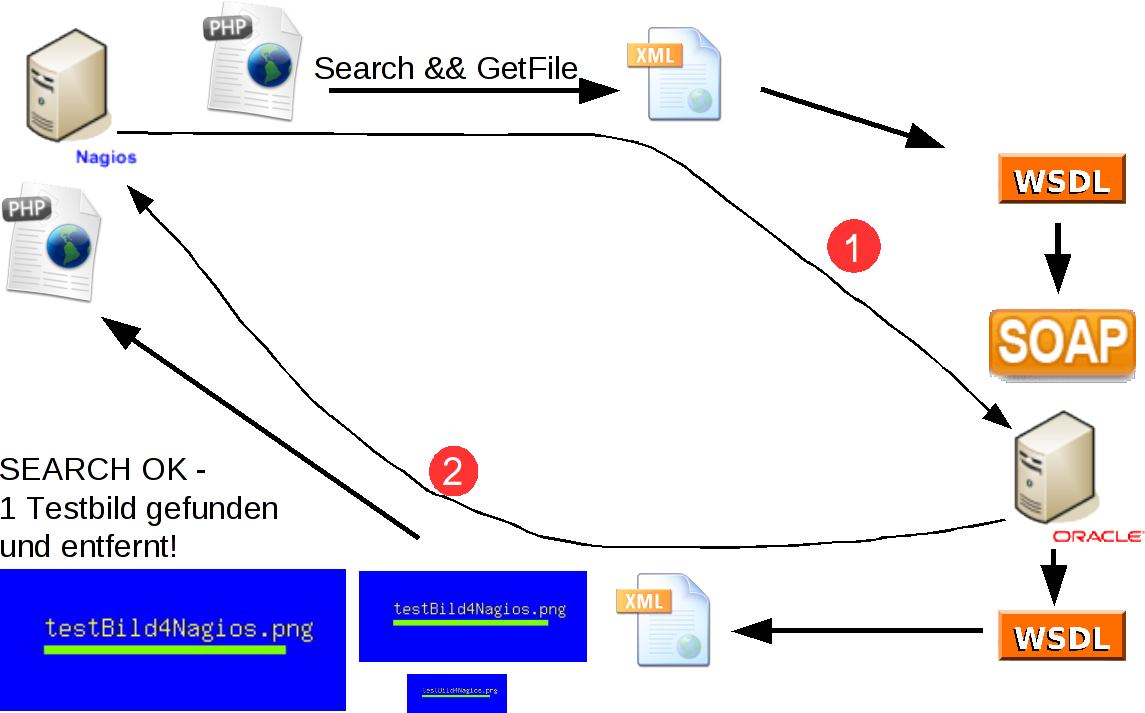
\includegraphics[width=0.93\textwidth]{bilder/wsdl-valid.png}}
		\caption{Technischer Ablauf der Benutzersimulation 2}
		\label{usersim2}
\end{figure}
%
\begin{itemize}
\item \url{http://www.w3schools.com/soap/default.asp} Web Services und SOAP
\item \url{http://www.w3schools.com/wsdl/wsdl_summary.asp} WSDL
\item max attempts bei Search erhöhen, da Auslastung der InboundRef -> möglichst keine/geringe False Positives -> auf Ausblick verweisen, Rahmenbedingungen müssen im Feld in der Praxis erst noch gefunden werden
\end{itemize}



